\documentclass{article}
\usepackage[utf8]{inputenc}
\usepackage{hyperref}

\usepackage{graphicx}
\usepackage{subcaption}

\graphicspath{ {./images/} }
\usepackage{wrapfig}

\usepackage{caption}
\captionsetup[figure]{font=footnotesize}

\usepackage[backend=biber,
bibencoding=ascii,
style=ieee,
citestyle=numeric,
sorting=ynt
]{biblatex}
\addbibresource{bibliography.bib}

\title{Collaborative Learning: \\
\normalsize Strategies and Platform Development
}
\author{Paul Baier}
\date{April 20, 2020}

\begin{document}

\maketitle

\section{Introduction}
A student response system (SRS) is a tool used in classrooms to get student feedback in real time. Typically it would be an online tool that teachers can set up with questions and present to students, and students can connect and answer the questions providing real time results. Gamification is the process of applying learning outcomes to games. The goal of this project is to create a fully customizable and programmable gamified SRS platform. We categorize such a system as a ``student response game'' (SRG). 

\subsection{Kahoot}
Our system is based off an existing commercial platform called ``Kahoot!''. Kahoot is a platform that allows teachers to write questions and organize them together to create a game called a ``kahoot''. When played, the teacher projects the questions to the students, as seen in figure \ref{fig:kahoot-question} and the students answer the questions on their own devices. The quicker a student answers the question, the more points they get. No points are awarded or subtracted for incorrect answers. After each question the results are displayed for that question and then the scoreboard with each player's cumulative score is displayed, as in figures \ref{fig:kahoot-post_question} and \ref{fig:kahoot-scoreboard} respectively. When the game is finished an animation plays and the final results are displayed as shown in figure \ref{fig:kahoot-final}.

\begin{figure}
    \centering
    \begin{subfigure}[b]{0.49\textwidth}
        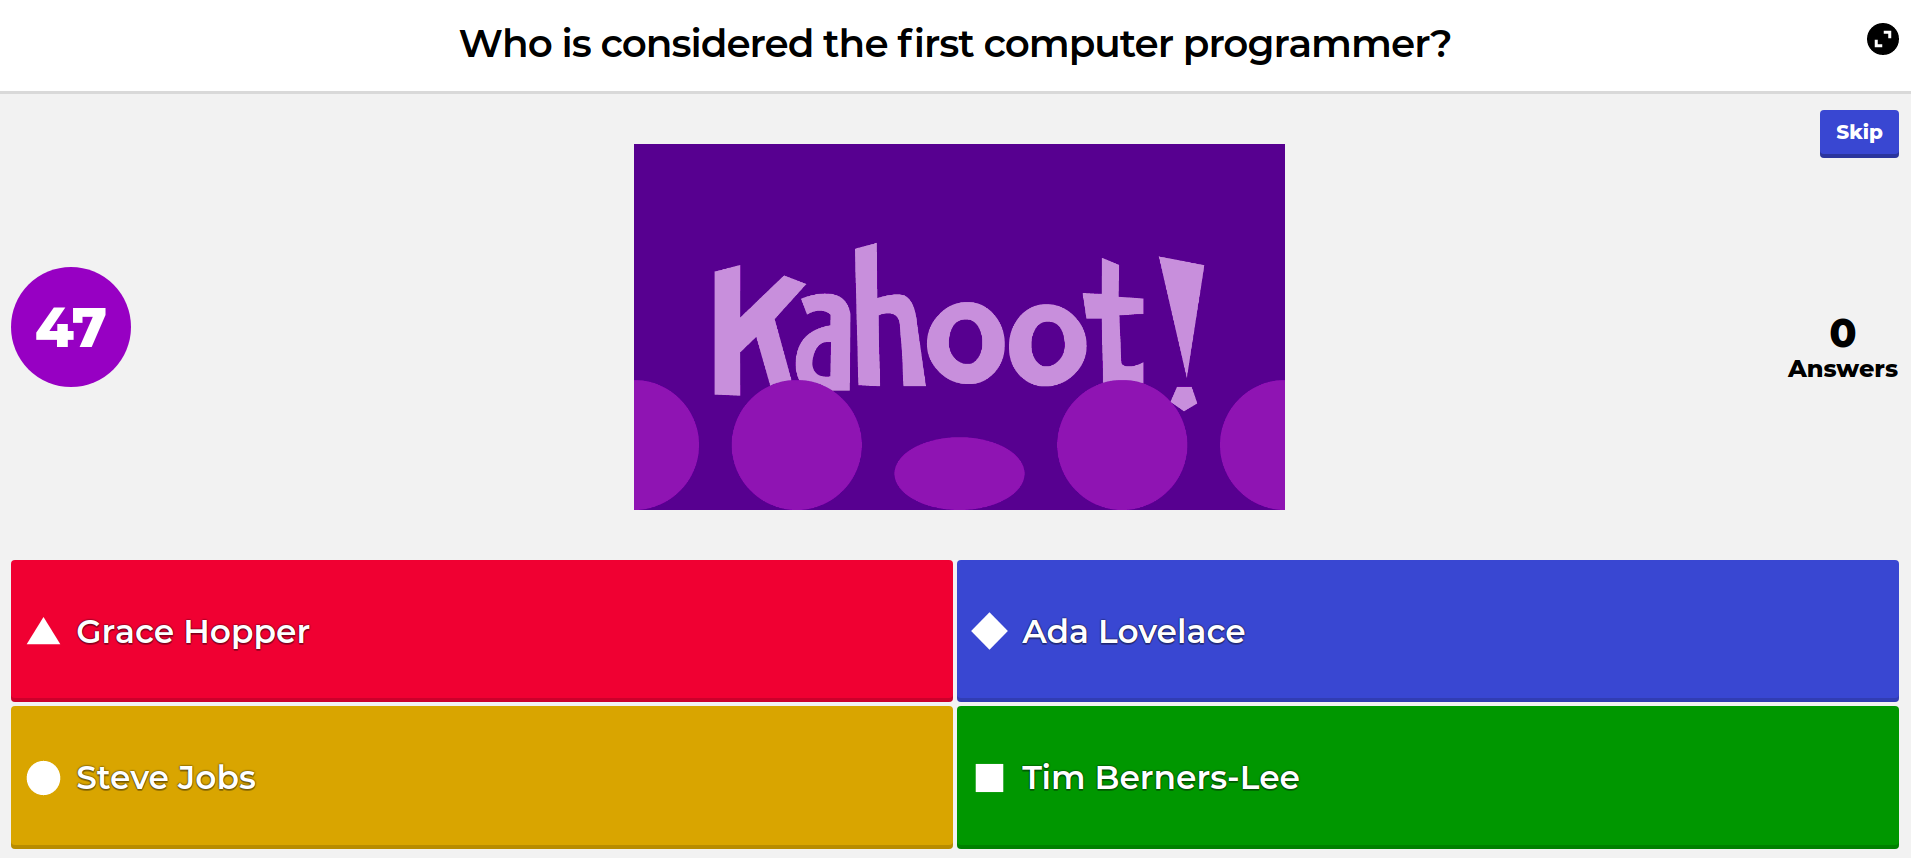
\includegraphics[width=\textwidth]{images/kahoot-question.png}
        \caption{Multiple Choice Question}
        \label{fig:kahoot-question}
    \end{subfigure}
    \begin{subfigure}[b]{0.49\textwidth}
        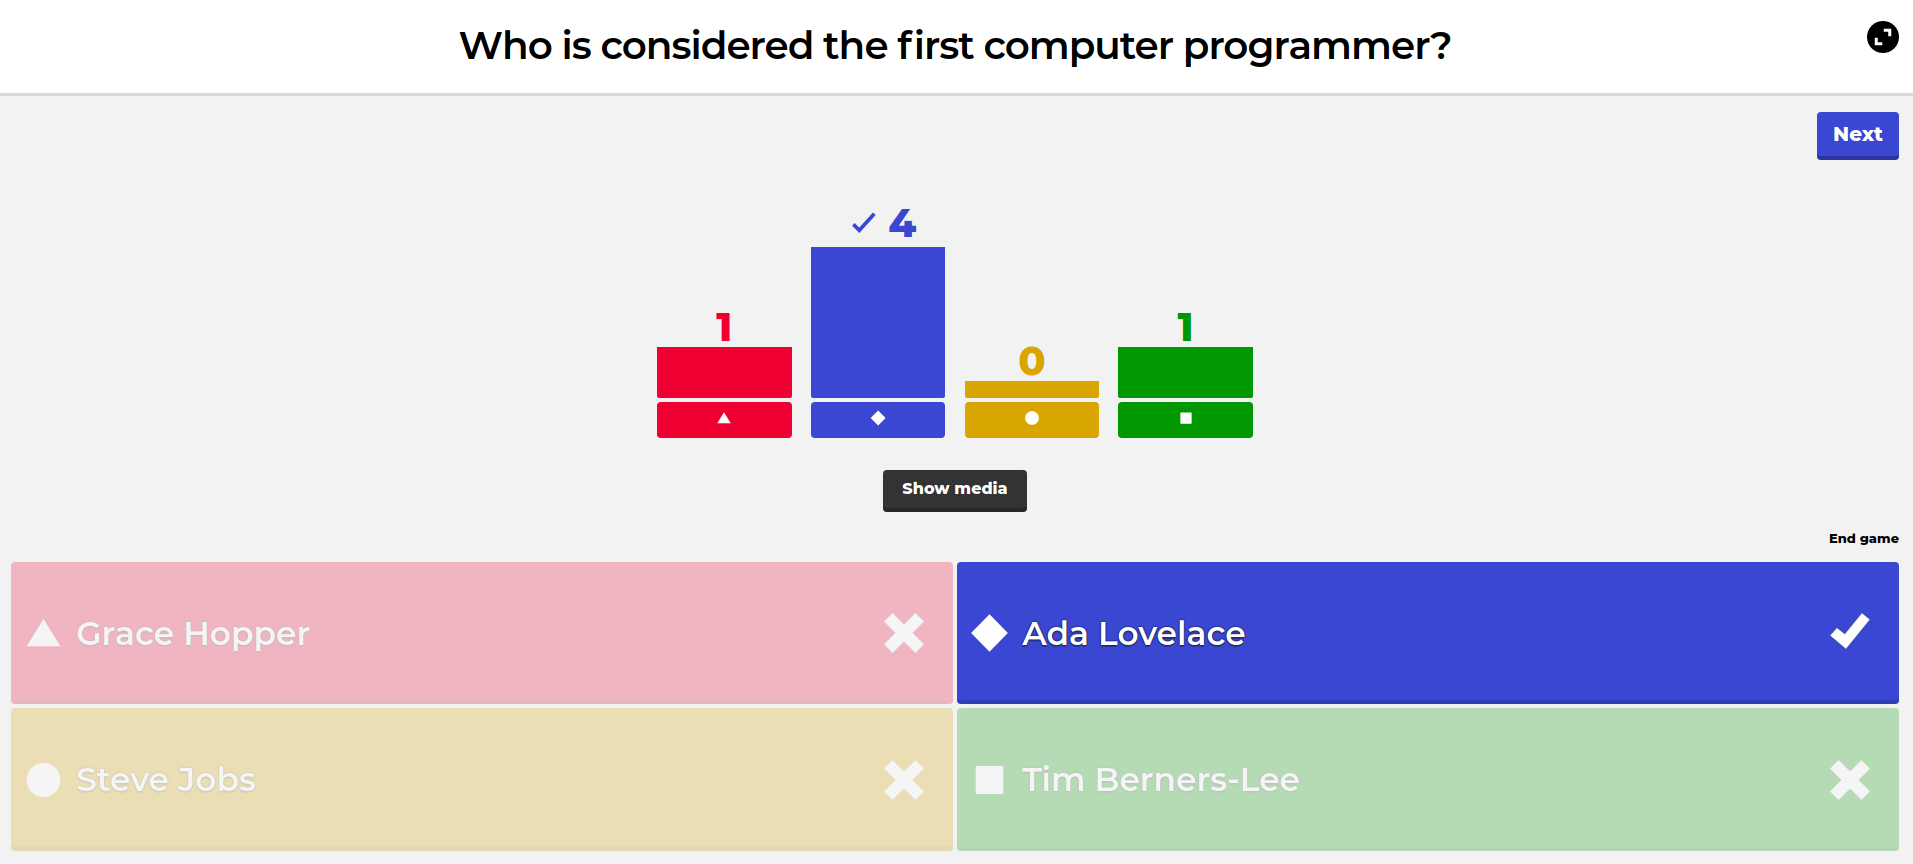
\includegraphics[width=\textwidth]{images/kahoot-post_question.png}
        \caption{Question Results}
        \label{fig:kahoot-post_question}
    \end{subfigure}
    \\
    \begin{subfigure}[b]{0.49\textwidth}
        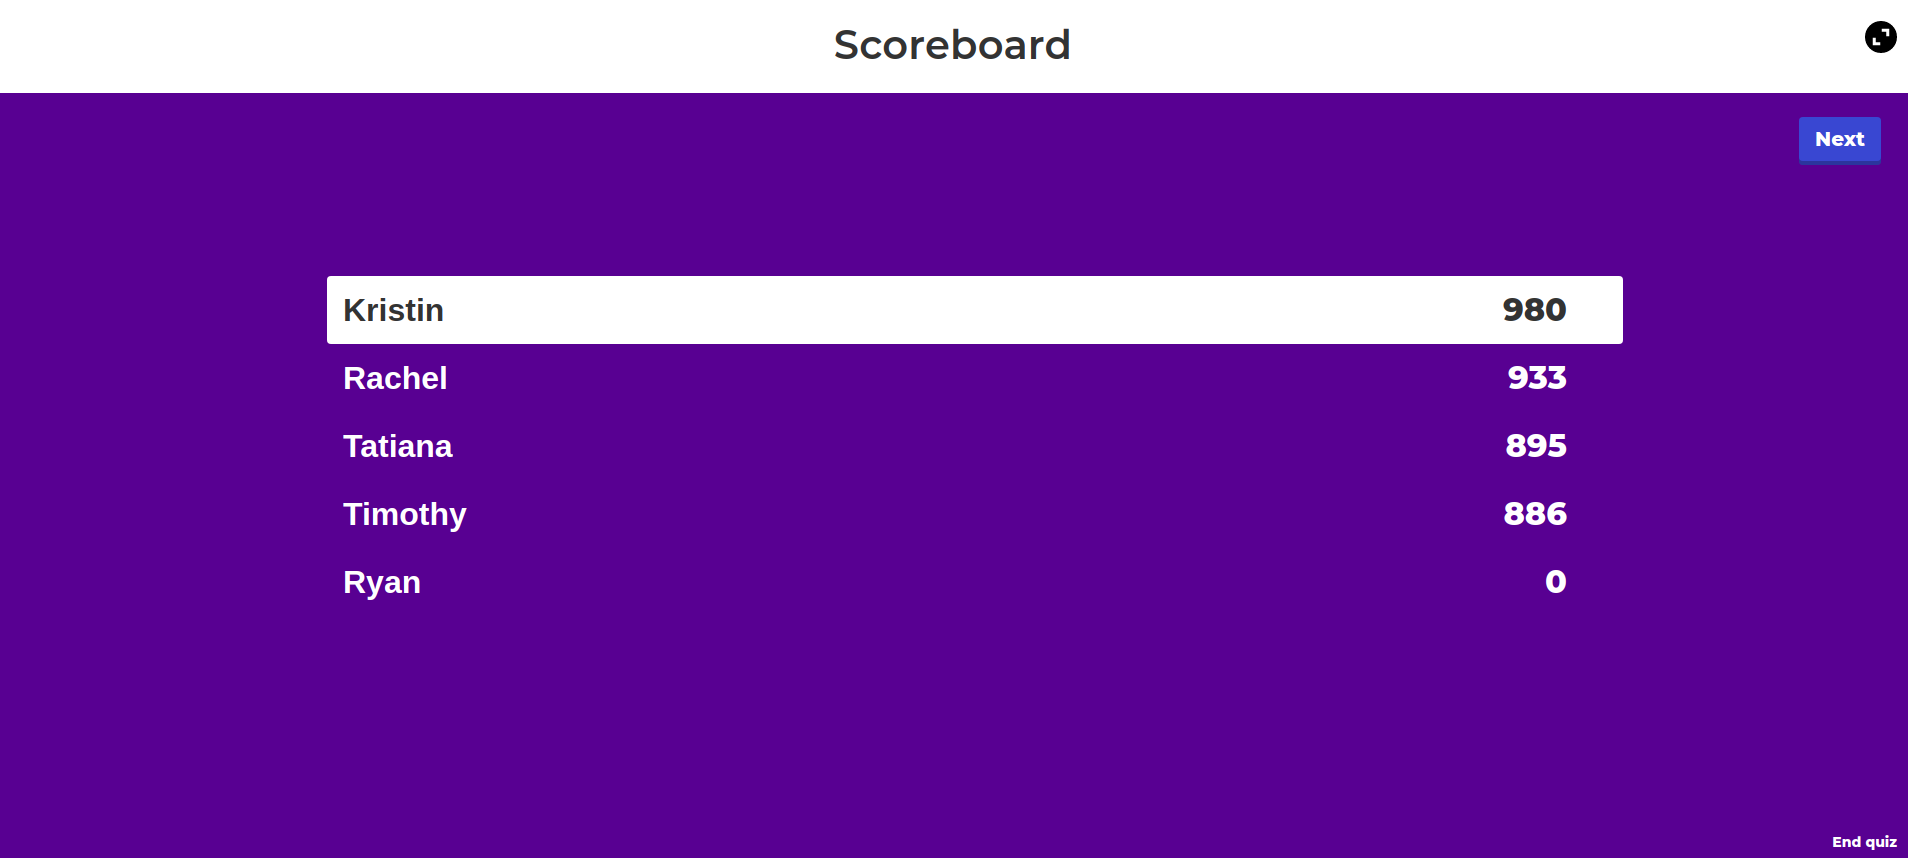
\includegraphics[width=\textwidth]{images/kahoot-scoreboard.png}
        \caption{Scoreboard}
        \label{fig:kahoot-scoreboard}
    \end{subfigure}
    \begin{subfigure}[b]{0.49\textwidth}
        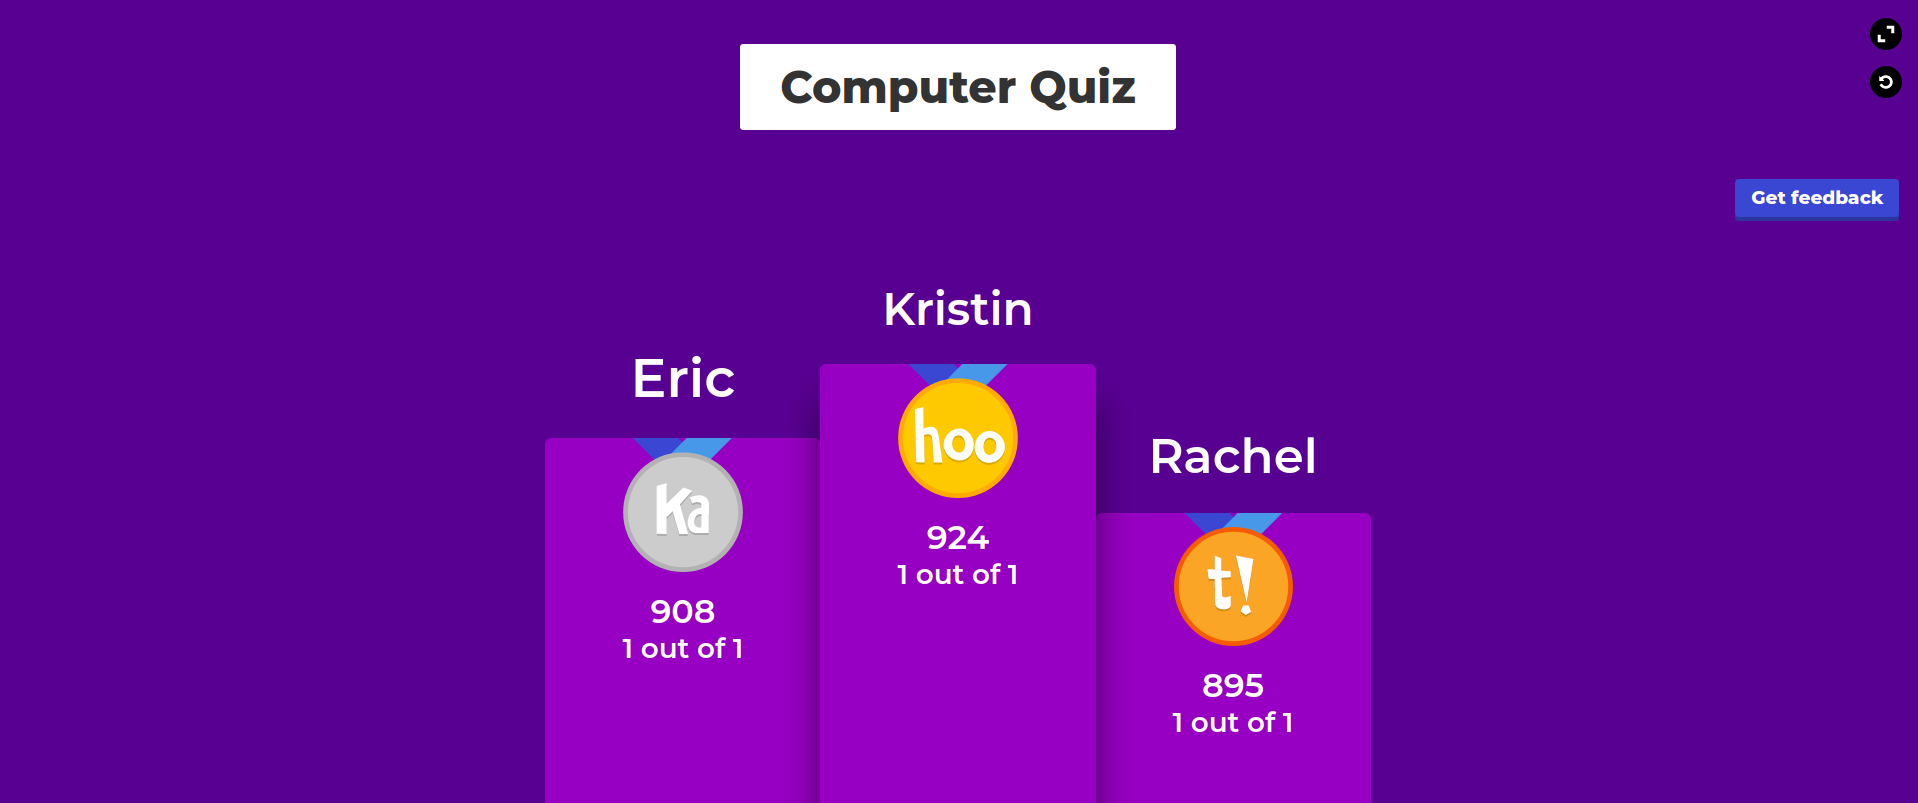
\includegraphics[width=\textwidth]{images/kahoot-finished.png}
        \caption{Final Results}
        \label{fig:kahoot-final}
    \end{subfigure}
    \caption{Kahoot Screens \cite{kahoot}}\label{fig:kahoot}
\end{figure}

When creating questions teachers are given six choices for the type of question they want to create: multiple choice, true/false, open-ended (players write in their answer), puzzle (players need to order the answers correctly), poll (no points awarded, simply polling the players), and slide, which is not a question but rather a screen with text to display more information. Each question has text and teachers are given the option to include a picture or YouTube video.
\smallskip

A Kahoot can be played live in the classroom or assigned to students to complete at their own pace. If assigned, the teacher needs to enter a due date and can set a few game options including randomize the questions, randomize the answers in each question, and use the question timer. Live games can be played in either classic mode, where students compete individually, or team mode. The difference between the two modes is that students share a device in team mode. Game options include randomizing the question and answers (like in the assigned option) and automatically moving through the questions instead of the teacher needing to click the ``next'' button as seen in figure \ref{fig:kahoot-scoreboard}.

\subsection{Motivation}
We decided to create a flexible, programmable SGR because we like the idea of Kahoot but find it limiting in the game options it offers. The idea originated with student collaboration in mind - creating a platform like kahoot but more collaborative - because Kahoot's team mode leaves a lot to be desired. As we iterated over different designs and features to include we eventually arrived at the idea that users (teachers) should be able to program the game and its features to do whatever they want it to do. With this concept at the core of our platform, we designed an open system with all of the game logic and data exposed to the user. There are default behaviors built into the system for those that want a hassle free experience, but for the more ambitious and/or particular, the default behavior can be overridden and programmed in any number of different ways.  

\section{Literature Review}
In order to identify prior work in the area of educational games we looked at roughly 2000 proceedings from the Frontiers in Education (FIE) conference from 2015-2019. We started our search with the word ``kahoot'' because our platform's functional design is based off of Kahoot. Within the search results we identified other platforms mentioned that were similar to Kahoot (and therefore also similar to our platform) and recursively searched for those other platforms as well within the proceedings. This search method allowed us to determine other popular platforms researchers were testing that are comparable to Kahoot as well as other SRS/SRG platforms in development. Our search revealed some of the most popular and relevant SRGs currently in production in addition to Kahoot are Socrative \cite{socrative}, Quizizz \cite{quizizz}, and Quizlet \cite{quizlet}. There were also two platforms in development by researchers called Quipid \cite{quipid} and Dysgu \cite{dysgu}.

\subsection{Quizizz}
Of the existing platforms Quizizz most resembles Kahoot and has many customizable features. The main difference between it and Kahoot or our platform is that students move through the quiz at their own pace, limited by the time assigned to each question.
\smallskip

To get started a teacher can either choose a preexisting quiz from a library of quizzes organized by topic or they can create their own. If they choose a pre-made quiz, they can use it as is or copy and edit it to their liking. If they choose to create a new quiz, they can search through existing quizzes for questions in addition to creating their own.
\smallskip

Question types include multiple choice, checkbox (select all the correct answers), fill-in-the-blank, polls, and open-ended (the last two are ungraded but marked as correct in reports). For each question the teacher can specify the amount of time the student has to answer. Scores for answering a question correctly are determined in part by the time it took the student to answer relative to the time length of the question. However, the timer can be disabled in which case the time factor would not be considered when scoring a question.
\smallskip

Once the quiz is made there are three game modes: team, classic, and test. We will only look at team and classic modes as test mode is beyond the scope of our work.
\smallskip

Team mode, as the name suggests, organizes students into teams. In classic mode each student competes by themselves. The main difference between the two modes is that the number of teams needs to be specified by the teacher in team mode and the team scores are based on the cumulative results of the team members. Both team and classic mode share similar gameplay settings. A teacher is able to toggle the timer on or off for the game, shuffle the questions, shuffle the answer options, and allow for a ``redemption question'' where students are able to retry missed questions. There are also memes that show up between questions that the teacher can toggle off for the game or the student can toggle off for their own experience. Another option teachers have is to either show the correct answer to the student in the game after they answer, show only if the got the question right or wrong, or do not visually indicate a correct or incorrect answer (there is a noise that indicates correct or incorrect regardless of this setting).
\smallskip

Lastly Quizizz has a feature called ``Power-ups'' which ``are single-use abilities designed to increase engagement and participation'' \cite{quizizz}. Currently there are nine power-ups that are awarded sporadically to players. Once awarded, an icon appears on the student's screen and they can use it any time by clicking on the icon. An example of a power up is 50-50 which eliminates half of the incorrect answers. This entire system is available in both team and classic mode and can be disable before starting the game.
\smallskip

Described above are only some of the features offered on the Quizizz platform but they represent the most relevant when compared with our design.

\subsection{Socrative}
Socrative is a web application focused on student engagement and tracking. It offers a number of features outside of the scope of our application, however one of its activities, called ``Space Race'', is comparable.
\smallskip

Space Race is a quiz-like game where students are asked a series of questions prearranged by the teacher. Figure \ref{fig:socrative-space-race} shows how student progress is tracked by little rocket ships (or other icons) that move across the teacher's dashboard when a question is answered correctly. The goal is to be the first individual or team to have their rocket reach across the screen.
\smallskip

\begin{figure}
    \centering
    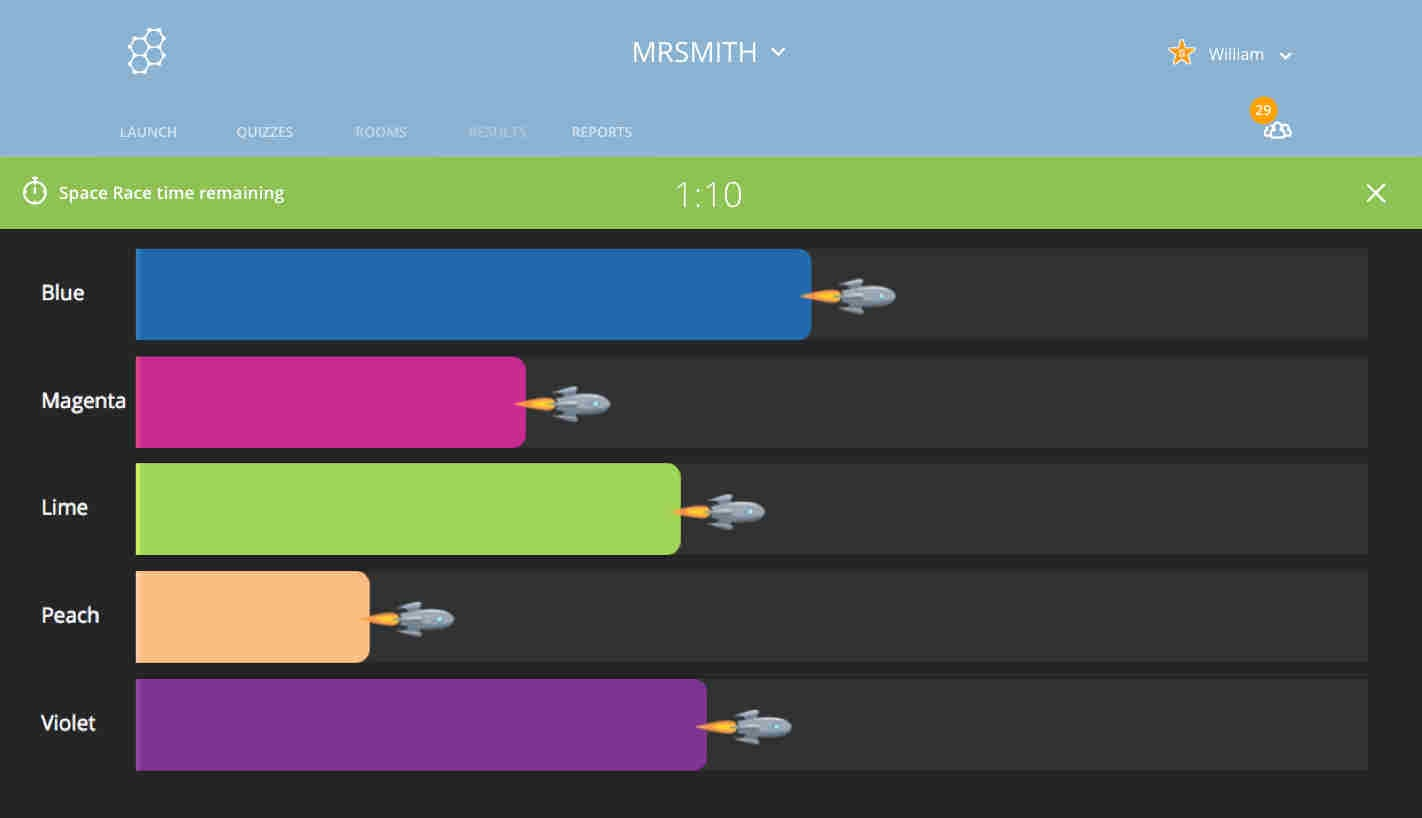
\includegraphics[width=0.9\textwidth]{images/socrative-space_race.jpg}
    \caption{Socrative Space Race \cite{socrative}}
    \label{fig:socrative-space-race}
\end{figure}

Quizzes can be made of multiple choice, true/false, and short answer questions. Other quiz options include the number of teams, how the players are assigned to teams (auto-assigned or student's choice), if the quiz is timed, shuffle the questions, shuffle the answers, show question feedback, show the final score, and if questions can only be attempted once.

\subsection{Quizlet}
Like Socrative, Quizlet is a web application that offers many features to its users. It provides students and teachers with the tools to create interactive study materials based on ``sets'', which are essentially digital flashcards. Each set is made up of any number of ``cards'' which contain a term ``side'' and a definition ``side''. Teachers and students can input the term and definition for their cards and create their own sets.
\smallskip

While most of the features offered by Quizlet do not overlap with our platform there is one, called ``Quizlet Live'', that is similar.
\smallskip

Quizlet live is a game that asks students multiple choice questions. Figure \ref{fig:quizlet-live} is the view from the teacher's dashboard that tracks student progress in real time. The teacher selects the set they want to use for the game and is able to choose between individual and team mode. Once selected the teacher is given the option for the questions to be generated based on the term side of the card or the definition side. The game ends for everyone when the first individual or team answers all of the questions correctly. If a question is answered incorrectly the correct answer is shown and the individual or team starts back at the beginning. Questions are randomly displayed to each player/team. In individual mode there are always four answer options shown in a random order, three of which are answers for other questions in the set.

\begin{figure}
    \centering
    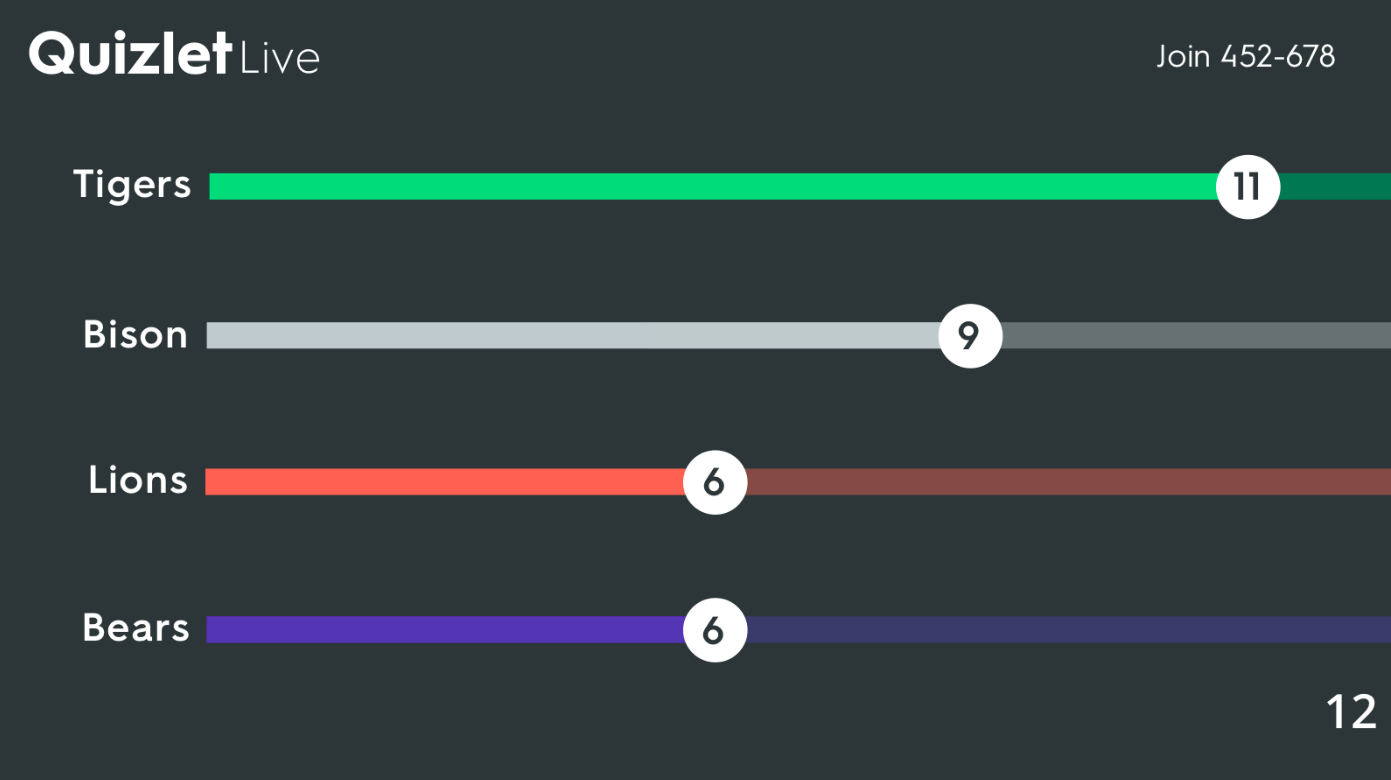
\includegraphics[width=0.8\textwidth]{images/quizlet-live.png}
    \caption{Quizlet Live Dashboard \cite{quizlet}}
    \label{fig:quizlet-live}
\end{figure}

In team mode the number of teams is automatically generated based on the number of players. Students are assigned to a team randomly and the teams can be shuffled by the teacher before the game starts. In the game, the answers to each question are split equally between each member of the team and always displayed on the screen. There are no wrong answers displayed in team mode.
\begin{wrapfigure}{l}{0.25\textwidth}
    \centering
    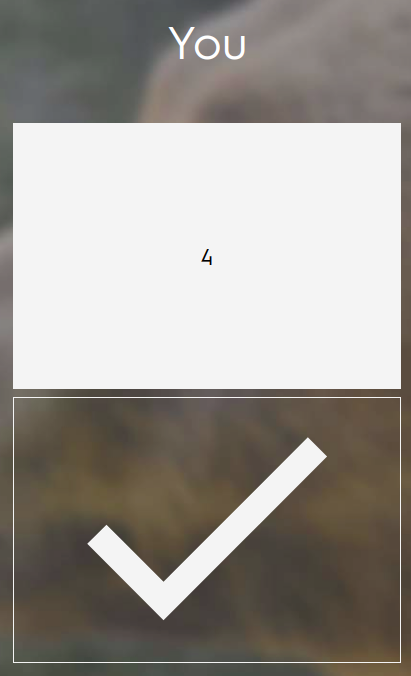
\includegraphics[width=0.15\textwidth]{images/quizlet-team.png}
    \caption{Quizlet Team View \cite{quizlet}}
    \label{fig:quizlet-team}
\end{wrapfigure}
Figure \ref{fig:quizlet-team} shows an example of one player's screen with two answer options, one of which has already been submitted correctly and replaced with a check mark. The other answer option, ``4'', will need to be used in an upcoming question.
\smallskip

To illustrate the point further, if there were 10 questions and two people on one team, then each person on that team would see five answers on their screen. Each answer is the answer to one of the questions but because the answers are divided across all team members, a player will not always have the answer to a question on their screen. It is up to the player with the correct answer to answer the question. Once the question is answered correctly a check mark appears where that answer used to be and the next question is displayed.

\subsection{Quipid}
A tool that was presented at the FIE 2017 conference is called Quipid. Its purpose is to provide students with rapid feedback on assessments and teachers with a simple way to create and assign assessments. It is not a game, so it does not directly relate to our platform, however it allows teachers to create custom questions and has a programmable element which makes it related and unique relative to other platforms we looked at.
\smallskip

Quipid uses Google Sheets and Google Forms as a front end for the platform. The teacher uses Google Sheets to formulate questions and organize them into a quiz. The quiz is exported to a Google Form where the students go to take the quiz. Once complete, the students are able to see their score along with feedback. Teachers can also see real time results once a student submits their work.
\smallskip
\begin{wrapfigure}{r}{0.25\textwidth}
    \centering
    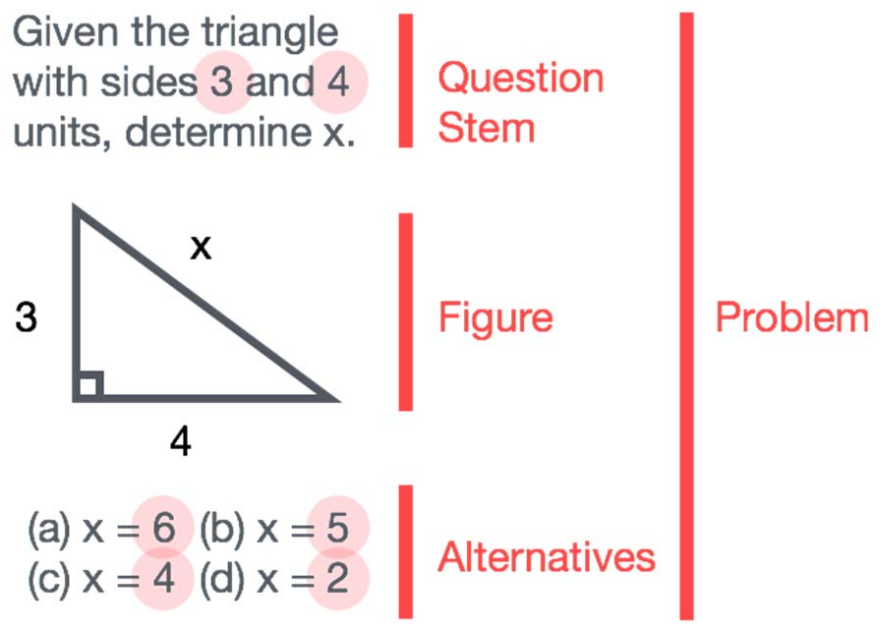
\includegraphics[width=0.25\textwidth]{images/quipid-problem.png}
    \caption{Quipid Problem Structure \cite{quipid}}
    \label{fig:quipid-problem}
\end{wrapfigure}
\indent A main goal for Quipid is to provide teachers with an easy way to assess students. Google Sheets is the backbone to achieving this goal. Quipid is designed with two sheets, a ``Problem'' sheet and a ``Formulation'' sheet. The Problem sheet is a library of questions and is linked to the formulation sheet. As figure \ref{fig:quipid-problem} shows, a problem is made up of three parts: a ``question steam'', an optional ``figure'', and ``alternatives'', which are the multiple choice options for the question. The link between the formulation sheet and the problem sheet allows the formulation sheet to be programmed in such a way that when a teacher changes the parameters in the question stem, the alternatives are automatically updated.
\smallskip

Along with the formulation sheet, Quipid offers more programmability simply by virtue of using Google's G Suite (Google Sheets and Google Forms). Part of G Suite is a scripting language called Google Apps Script. This allows the user to program the Sheets and Forms with virtually infinite possibilities. Quipid leverages Apps Script to create the quiz in Google Forms based on the questions in Google Sheets, but a user of Quipid could program the tool to do any number of different tasks including integrating with third party tools, at which point the possibilities would be endless.  

\subsection{Dysgu}
The last work, Dysgu, is a concept more than an application. It was presented at FIE 2018 in a ``work in progress'' paper. It is presented as a collection of high level ideas without any concrete implementation. We mention it here because it is a platform in development with gamification features and some interesting ideas on student engagement.
\smallskip

Dysgu is described as an application for teachers to assign activities to students and track their progress. Students can sign in, interact with each other, and complete the assignments. There are three notable gamification features presented: scores and points, badges, and social awareness.
\smallskip

The paper describes the difference between scores and points as ``Scores are utilized to calculate student’s grade, whereas, points are used as currency in the system'' \cite{dysgu}. All students receive scores for completing activities, but they can earn points by achieving certain goals within the activities, such as being the first to complete an activity. The points earned can then be used in various ways throughout the system, like a time extension on an activity. 
\smallskip

Badges are similar to points. They are awarded for certain accomplishments and unlock features for the student like getting a sneak peek into an activity.   
\smallskip

The social aspect of the platform allows students to see how they are doing relative to the rest of the class. While everything is done anonymously, certain general statistics are made available to each student. For example each student can see the number of students to have completed an activity and each student will know which place they are in relative to their points. Also each student will be able to see the others' badges. 

\section{Design}
	\subsection{Languages}
		\subsubsection{Python}
		\subsubsection{Django}
\section{Development}
\section{Features}
\section{Future Work}

\printbibliography[title={Bibliography}]


\end{document}

